\documentclass[]{article}
\usepackage{hyperref}
\usepackage{multirow}
\usepackage{float}
\usepackage{textcomp}
\usepackage{graphicx}
\usepackage{float}
% Title Page
\title{Low-Comotovation: System Design Document}
\author{Michael Ghaben}
\date{}

\begin{document}

\maketitle
\tableofcontents
\titlepage

\subsection{Versioning \& Authorship}
Version 0.1
\newline
Low-Comotovation \textcopyright

\raggedright
Software Design Specification: Low-Comotovation \\
Status: Preliminary Release: Software Design Review

\subsection{References}
During the development of this document, IEEE 1016 was utilized.

\subsection{Purpose}
This document will specify the architecture and design of the Low-Comotovation train system. It shall discuss the structural and design and considerations of the train system and the accompanying subsystems of the train system. It shall also detail design considerations in vital subsystems.

\subsection{Stakeholders \& Concerns}
The stakeholders of this document are anticipated to be the following:
\begin{itemize}
	\item Future Design Teams: Future design teams are anticiapted to utilize this document to guide their usage of the track controller system
	\item Pittsburgh Rail Company: The rail company utlizing the Software Design Specification (SDS) to guide the development of physical systems associated with the software
\end{itemize}

Future design teams associated with the continued development beneift from increased documentation of the original system by allowing for more efficient software design procedures in future revision by potentially unrelated developers.

The benefits to the Pittsburgh Rail Company from  a detailed software design specification are twofold. First, a detailed SDD provides developers of railway hardware the information required to produced a paired system. Second, a documented SDD allows the Pittsburgh Rail Company to evaluate the designs ability to meet specifications for vitality.

\section{Introduction}
To ensure safe, predictable, and reliable operation of the system, there are three primary considerations:
\begin{enumerate}
	\item \emph{Vitality:} Vitality of a system within this document referse to a safety-critical system.
	\item \emph{Testability:} Any system implemented must be easily tested to ensure reliability
	\item \emph{Modularity:} Any system designed must reuse code wherever possible
\end{enumerate}

\section{System Design Use Cases}
In this section, we detail the use cases of each subsystem. The use case of each subsystem is accompanied by brief descriptions of the use cases.

\subsection{Track Model}
In this subsection, the use cases of the train model are provided.

\begin{figure}[H]
	\centering
	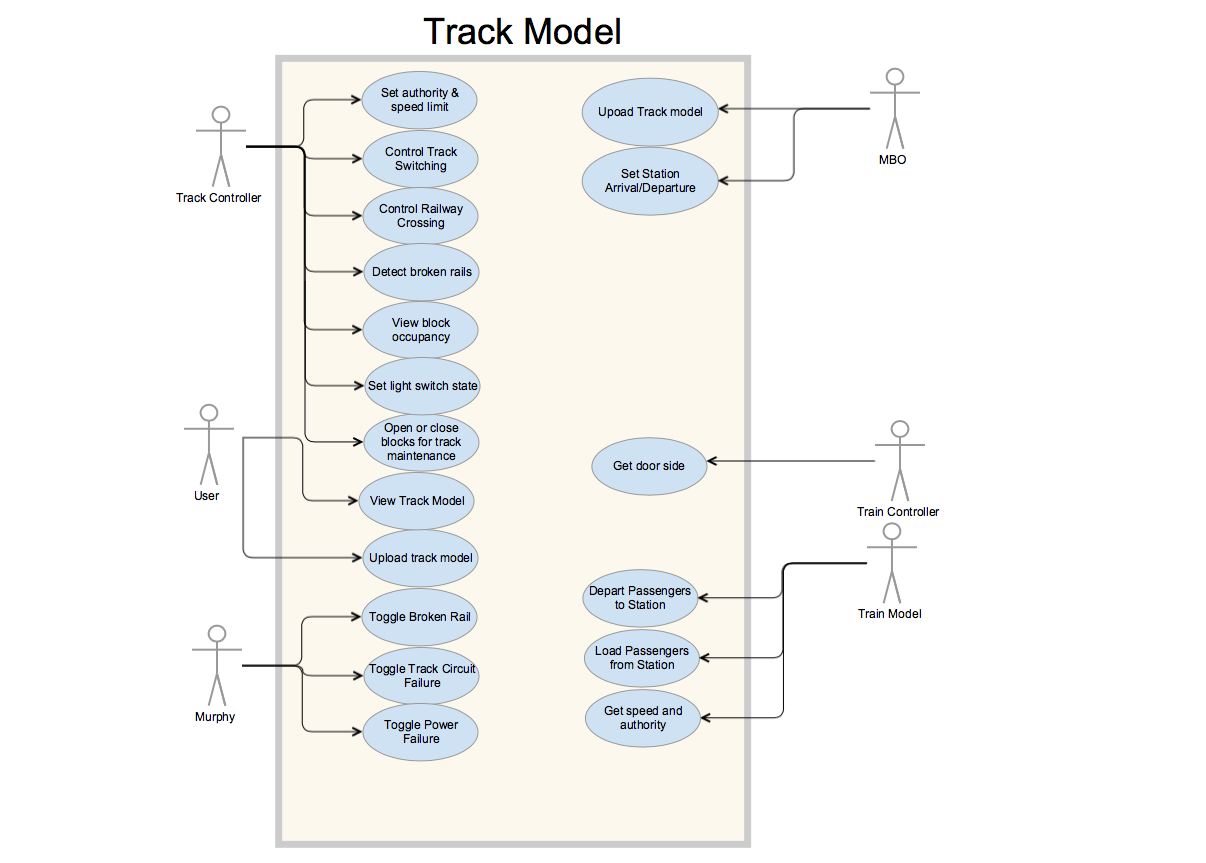
\includegraphics[scale=.3]{trackmodelusecase.png}
	\caption{Track model use case diagram}
\end{figure}

\subsection{Track Controller}
In this subsection, the use cases of the track controller are provided.

\begin{figure}[H]
	\centering
	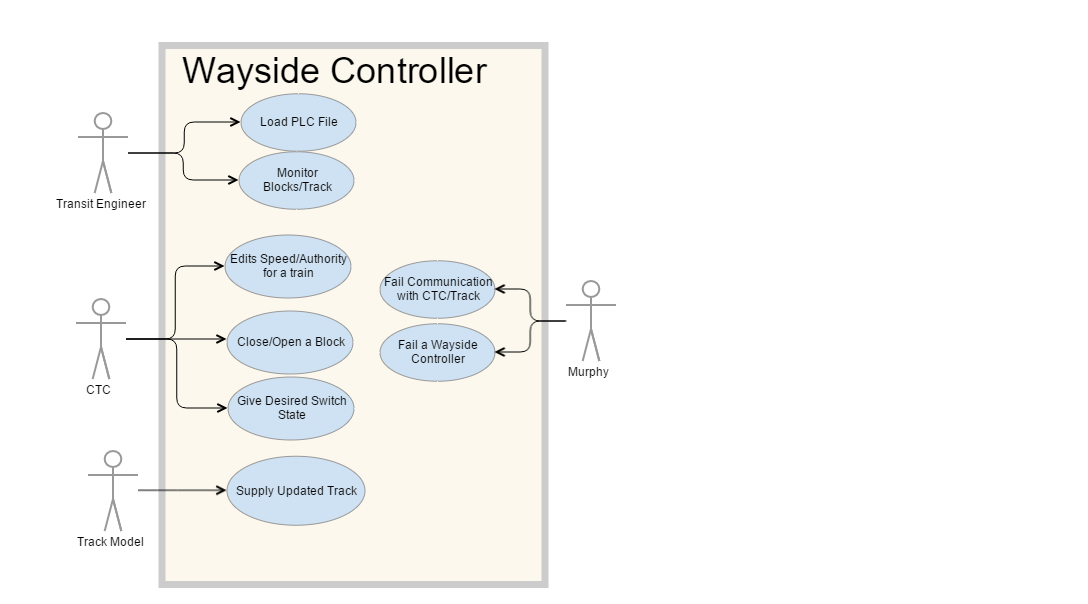
\includegraphics[scale=.3]{trackcontrollerusecase.png}
	\caption{Track controller use case diagram}
\end{figure}

\subsection{Train Model}
In this subsection, the use cases of the train model are provided.

\begin{figure}[H]
	\centering
	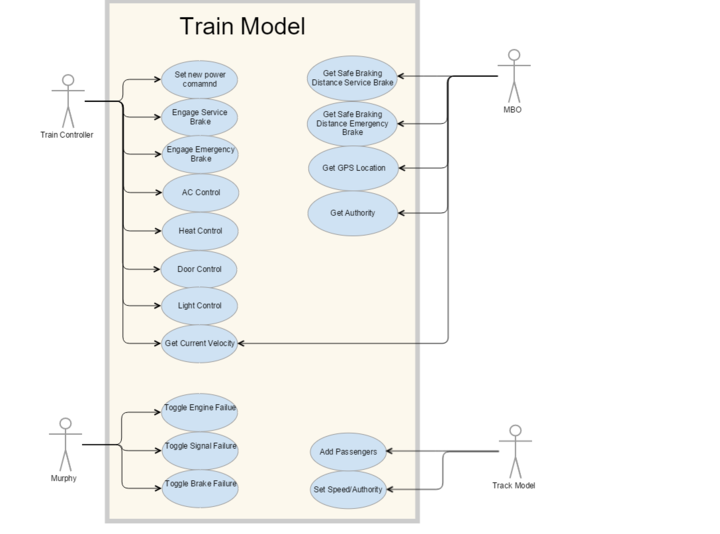
\includegraphics[scale=.3]{trainmodelusecase.png}
	\caption{Train model use case diagram}
\end{figure}

\subsection{Train Controller}
In this subsection, the use cases of the train controller are provided.

\begin{figure}[H]
	\centering
	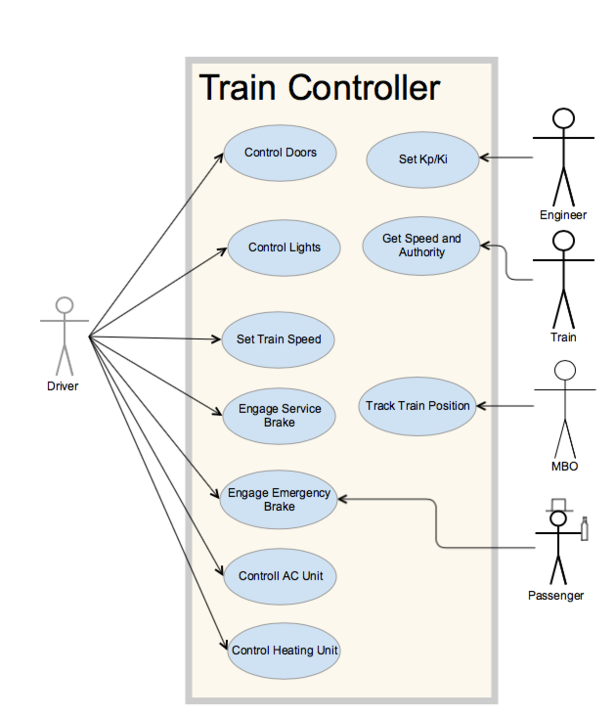
\includegraphics[scale=.2]{traincontrollerusecase.png}
	\caption{Train controller use case diagram}
\end{figure}

\subsection{Moving Block Overlay}
In this subsection, the use cases of the Moving Block Overlay (MBO) are provided.

\begin{figure}[H]
	\centering
	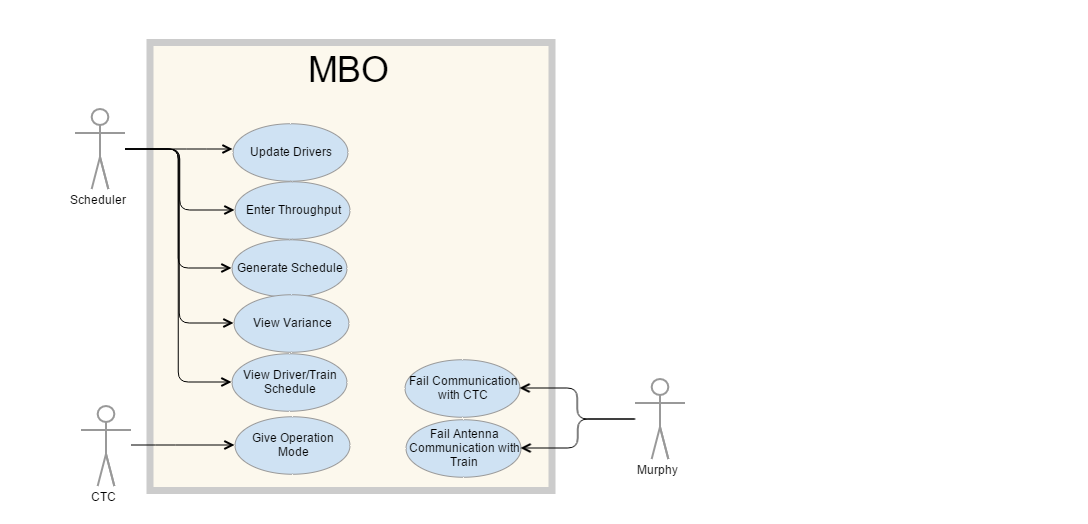
\includegraphics[scale=.2]{mbousecase.png}
	\caption{Train controller use case diagram}
\end{figure}
\begin{table}[H]
	\centering
	\caption{Update}
	\begin{tabular}{|l|l|}
		\hline
		Actors & \parbox[t]{10cm}{Scheduler} \\ \hline
		Description & \parbox[t]{10cm}{The Scheduler is able to update the list of drivers. This will change whether or not a driver is able to be scheduled.} \\ \hline
		Data &  \parbox[t]{10cm}{filename} \\ \hline
		Stimulus &  \parbox[t]{10cm}{Click drivers button} \\ \hline
		Response & \parbox[t]{10cm}{Loops through a CSV file to add all the drivers to the list of drivers. When adding a driver, a driver object will be created with the entered properties. This object will then be added to the Driver Schedule where it can be accessed as part of the list.}\\ \hline
		Comments & \parbox[t]{10cm}{There will be a default file so that it can be saved between sessions.}  \\ \hline
	\end{tabular}
\end{table}

\begin{table}[H]
	\centering
	\caption{Enter Throughput}
	\begin{tabular}{|l|l|}
		\hline
		Actors & \parbox[t]{10cm}{Scheduler} \\ \hline
		Description & \parbox[t]{10cm}{The Scheduler enters the number of trains they would like to be on the track at a certain point in time.} \\ \hline
		Data &  \parbox[t]{10cm}{number of trains} \\ \hline
		Stimulus &  \parbox[t]{10cm}{Click submit button} \\ \hline
		Response & \parbox[t]{10cm}{The number of trains is entered by the scheduler. This is used to generate both the train and driver schedules for both MBO and FB modes.}\\ \hline
		Comments & \parbox[t]{10cm}{}  \\ \hline
	\end{tabular}
\end{table}

\begin{table}[H]
	\centering
	\caption{View Train/Driver Schedule}
	\begin{tabular}{|l|l|}
		\hline
		Actors & \parbox[t]{10cm}{Scheduler, CTC} \\ \hline
		Description & \parbox[t]{10cm}{Scheduler can see a list of all  trains, as well as their station arrival times. Scheduler can see a list of all current drivers, as well as their corresponding break times and current train. } \\ \hline
		Data &  \parbox[t]{10cm}{train ID, arrival times, driver name, ID, break times} \\ \hline
		Stimulus &  \parbox[t]{10cm}{Updates triggered by clock} \\ \hline
		Response & \parbox[t]{10cm}{Two tables will be displayed, one for the train schedule, and one for the driver schedule. The train schedule will list IDs as the rows and station names as the columns. Each cell will contain the time that train will arrive at that station. The driver schedule will what train they are on at what times. It will also show whenever they start and stop work and when they are on breaks.}\\ \hline
		Comments & \parbox[t]{10cm}{The table that is displayed will automatically update itself when triggered by the clock.}  \\ \hline
	\end{tabular}
\end{table}

\begin{table}[H]
	\centering
	\caption{View Variance}
	\begin{tabular}{|l|l|}
		\hline
		Actors & \parbox[t]{10cm}{Scheduler} \\ \hline
		Description & \parbox[t]{10cm}{Scheduler can see a list of all  trains, as well as their corresponding speed and current position. The suggested speed and authority will be displayed as well as the variance between the two.} \\ \hline
		Data &  \parbox[t]{10cm}{train ID, speed, suggested/actual position/authority, variance} \\ \hline
		Stimulus &  \parbox[t]{10cm}{Updates triggered by clock} \\ \hline
		Response & \parbox[t]{10cm}{In Fixed Block mode the current block will have to be kept track of based on past block occupancy. In MBO mode the position can be gotten through GPS.}\\ \hline
		Comments & \parbox[t]{10cm}{In Fixed Block mode the position is denoted as the current block. In MBO mode the position is denoted as the current block and the distance into that block.}  \\ \hline
	\end{tabular}
\end{table}

\begin{table}[H]
	\centering
	\caption{Generate Schedules}
	\begin{tabular}{|l|l|}
		\hline
		Actors & \parbox[t]{10cm}{Scheduler} \\ \hline
		Description & \parbox[t]{10cm}{When required a schedule will be generated based on the input data. This will then be displayed for the scheduler/CTC. It is used to dispatch trains and calculate a path for a train.} \\ \hline
		Data &  \parbox[t]{10cm}{number of trains, track data} \\ \hline
		Stimulus &  \parbox[t]{10cm}{On launch, change in number of drivers, clock triggered} \\ \hline
		Response & \parbox[t]{10cm}{A schedule will be generated for trains and drivers. It will have to take into account the mode of operation (MBO or FB), speed limits, track occupancy, drivers’ break times, and other variables.}\\ \hline
		Comments & \parbox[t]{10cm}{Can only happen in automatic mode - schedule will be either fixed block or MBO depending on dispatcher's selection of mode.}  \\ \hline
	\end{tabular}
\end{table}

\begin{table}[H]
	\centering
	\caption{Give Operation Mode}
	\begin{tabular}{|l|l|}
		\hline
		Actors & \parbox[t]{10cm}{CTC} \\ \hline
		Description & \parbox[t]{10cm}{The CTC sends the mode of operation whenever it is changed.} \\ \hline
		Data &  \parbox[t]{10cm}{mode} \\ \hline
		Stimulus &  \parbox[t]{10cm}{CTC changes the mode.} \\ \hline
		Response & \parbox[t]{10cm}{The mode is updated in the MovingBlockOverlay class. Any “shutdown” procedures to switch between modes are performed.}\\ \hline
		Comments & \parbox[t]{10cm}{The default mode will be manual.}  \\ \hline
	\end{tabular}
\end{table}

\begin{table}[H]
	\centering
	\caption{Fail Communication with CTC}
	\begin{tabular}{|l|l|}
		\hline
		Actors & \parbox[t]{10cm}{Murphy} \\ \hline
		Description & \parbox[t]{10cm}{Murphy breaks communication between CTC and MBO.} \\ \hline
		Data &  \parbox[t]{10cm}{communication failure} \\ \hline
		Stimulus &  \parbox[t]{10cm}{CTC clicks Fail Communication with MBO button.} \\ \hline
		Response & \parbox[t]{10cm}{Since scheduling will be unavailable without communication with the MBO, the CTC will be forced into manual mode and let the dispatcher know with a message.}\\ \hline
		Comments & \parbox[t]{10cm}{}  \\ \hline
	\end{tabular}
\end{table}

\begin{table}[H]
	\centering
	\caption{Fail Communication with Train}
	\begin{tabular}{|l|l|}
		\hline
		Actors & \parbox[t]{10cm}{Murphy} \\ \hline
		Description & \parbox[t]{10cm}{Murphy breaks communication between Train and wayside.} \\ \hline
		Data &  \parbox[t]{10cm}{communication failure} \\ \hline
		Stimulus &  \parbox[t]{10cm}{Click Fail Communication with Train button.} \\ \hline
		Response & \parbox[t]{10cm}{The MBO can no longer receive the GPS position of individual trains and is therefore unable to safely operate in MBO mode. So a transition must be made to either Fixed Block mode or to manual mode.}\\ \hline
		Comments & \parbox[t]{10cm}{}  \\ \hline
	\end{tabular}
\end{table}

\subsection{Centralized Train Control}
In this subsection, the use cases of the Centralized Train Control (CTC) are provided.
\begin{figure}[H]
	\centering
	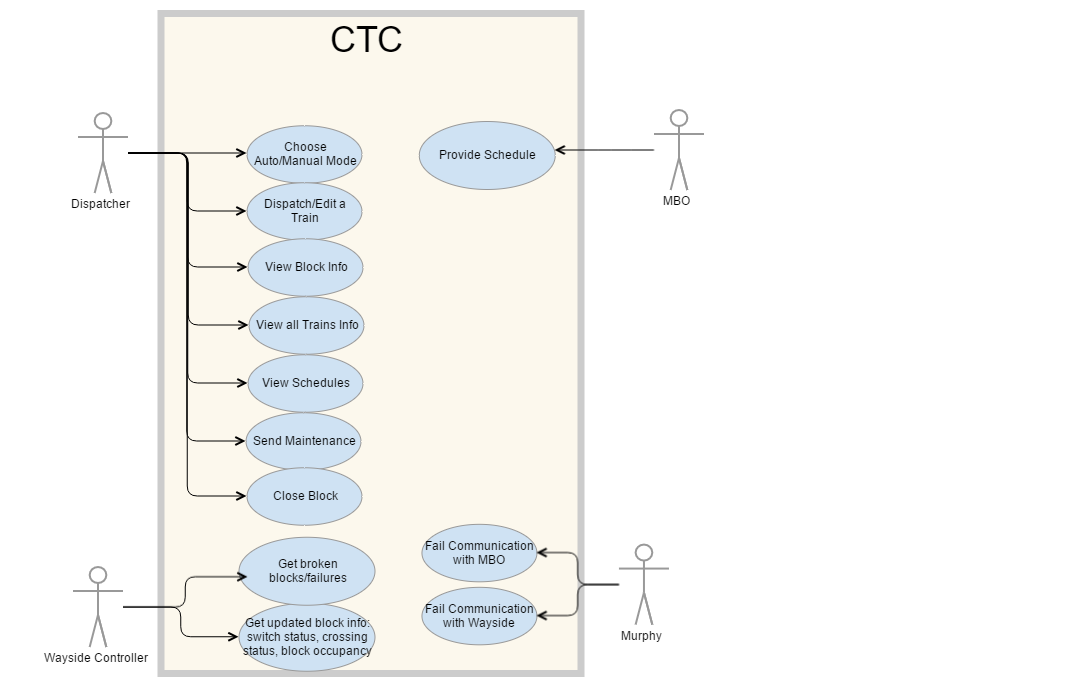
\includegraphics[scale=.15]{ctcusecase.png}
	\caption{Centralized Train Control use case}
\end{figure}

\section{Class Diagrams}
In this section, we detail the use class diagrams for each subsystem..
\subsection{Track Model}
\subsection{Track Controller}
\subsection{Train Model}
\subsection{Train Controlled}
\subsection{Moving Block Overlay}
\subsection{Centralized Train Controller}


\section{Sequence Diagrams}
In this section, we detail the sequence diagrams each subsystem.
\subsection{Track Model}

\begin{figure}[H]
	\centering
	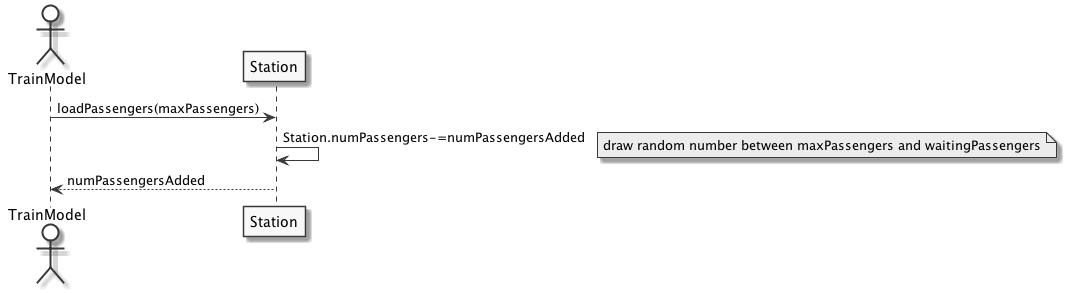
\includegraphics[scale=.3]{addPassengers.png}
	\caption{Add Passengers Use Case Diagram}
\end{figure}

\begin{figure}[H]
	\centering
	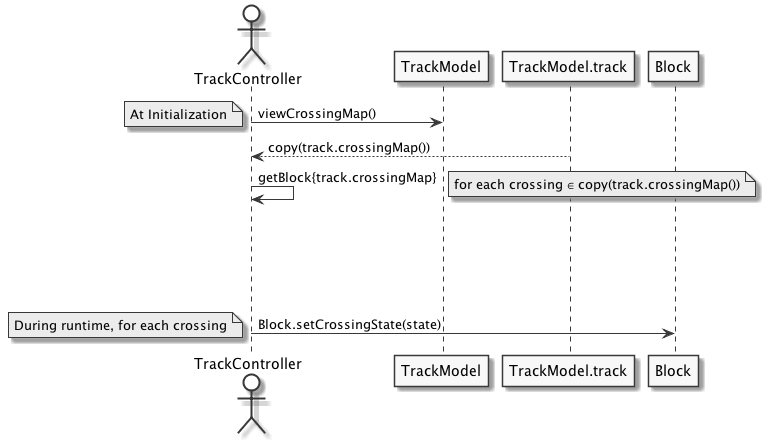
\includegraphics[scale=.3]{crossing.png}
	\caption{Toggle Crossing State Use Case Diagram}
\end{figure}

\begin{figure}[H]
	\centering
	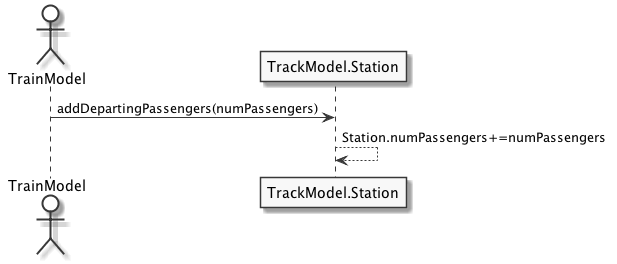
\includegraphics[scale=.3]{departPassengers.png}
	\caption{TDeparting Passengers to Station Use Case Diagram}
\end{figure}

\begin{figure}[H]
	\centering
	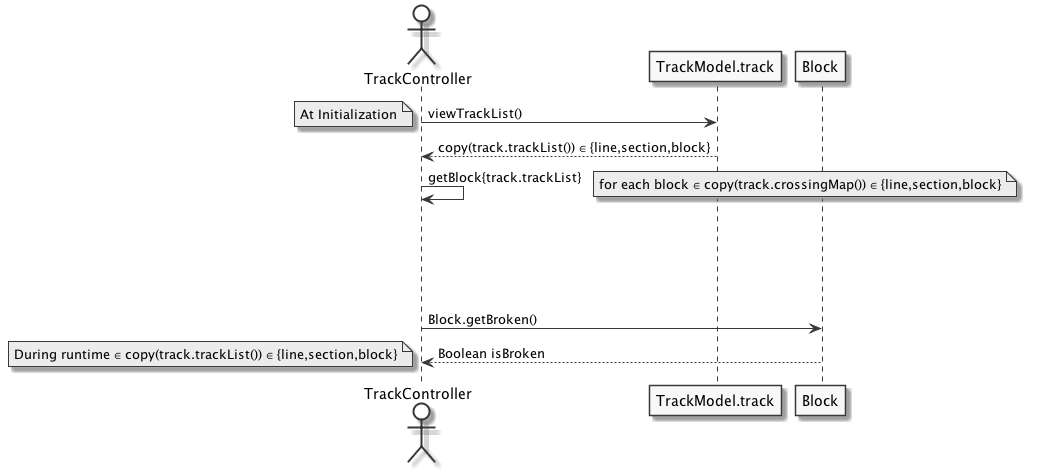
\includegraphics[scale=.3]{detectBroken.png}
	\caption{Detect Broken Rail Use Case Diagram}
\end{figure}

\begin{figure}[H]
	\centering
	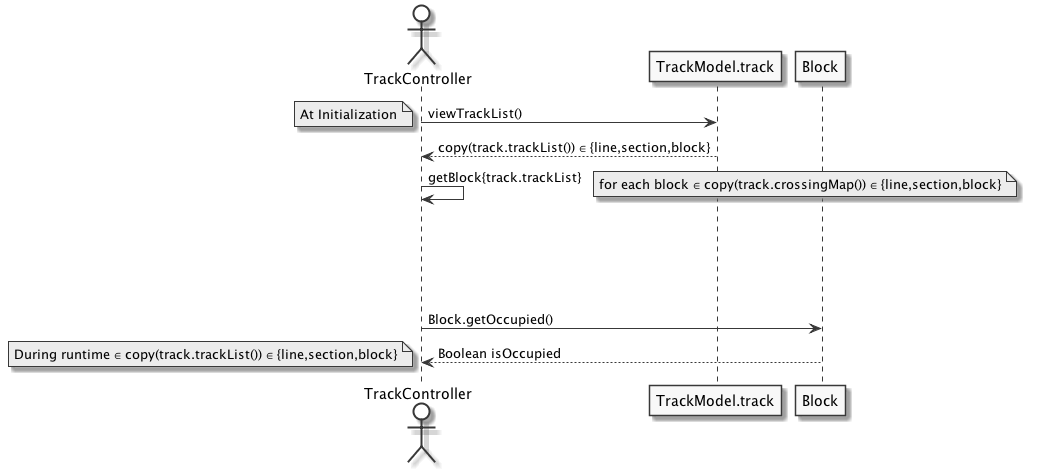
\includegraphics[scale=.3]{detectOccupied.png}
	\caption{Detect Block Occupancy use Case Diagram}
\end{figure}

\begin{figure}[H]
	\centering
	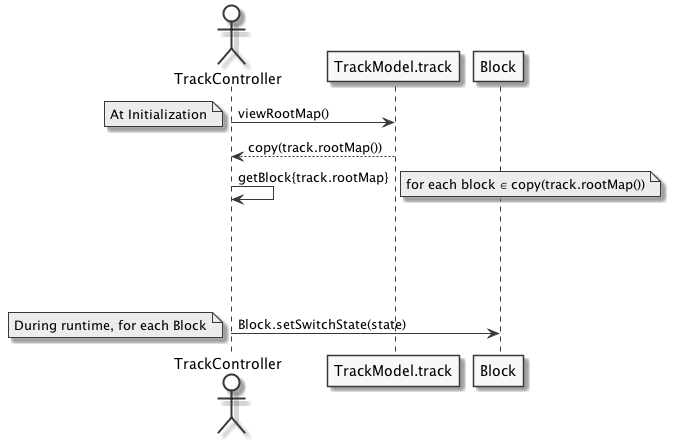
\includegraphics[scale=.3]{switching.png}
	\caption{Toggle Switching Use Case Diagram}
\end{figure}

\begin{figure}[H]
	\centering
	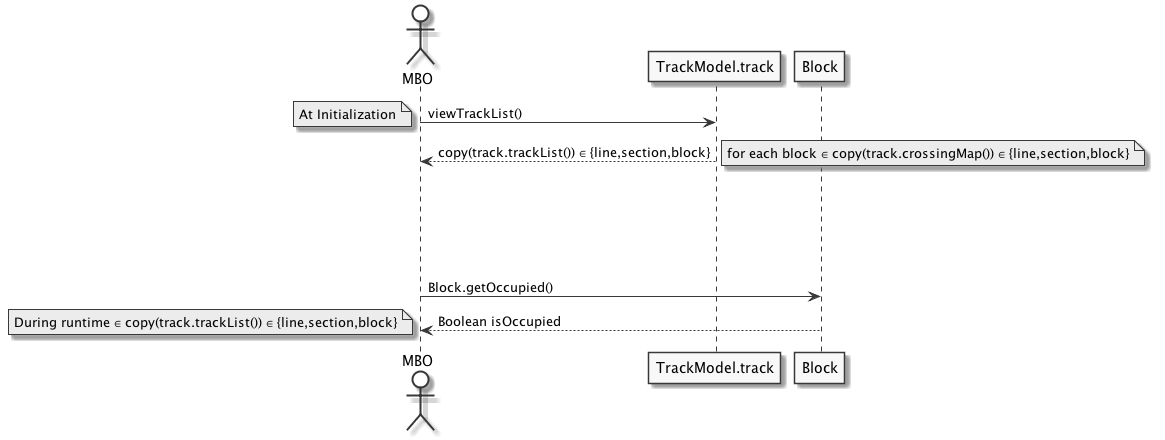
\includegraphics[scale=.3]{viewBlockOccupancy.png}
	\caption{View Block Occupancy Use Case Diagram}
\end{figure}

\begin{figure}[H]
	\centering
	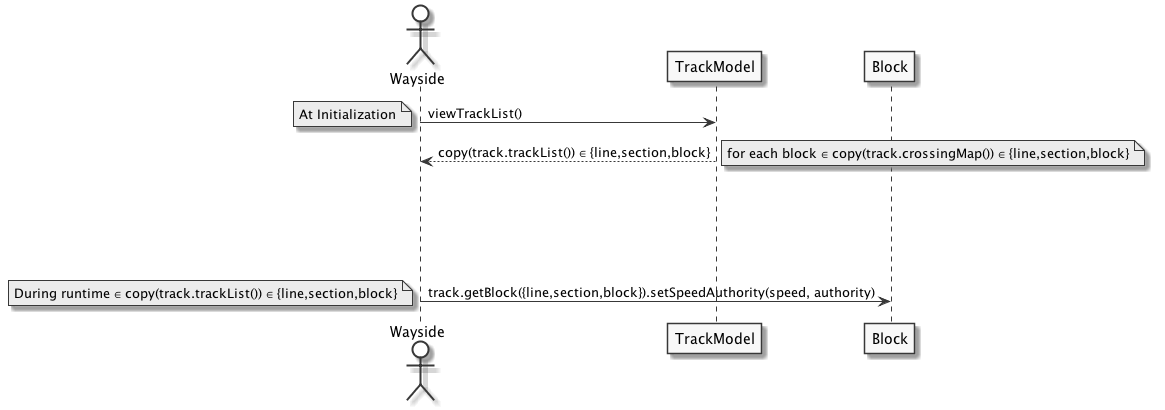
\includegraphics[scale=.3]{setSpeedAuthority.png}
	\caption{Set Speed and Authority use Case Diagram}
\end{figure}

\begin{figure}[H]
	\centering
	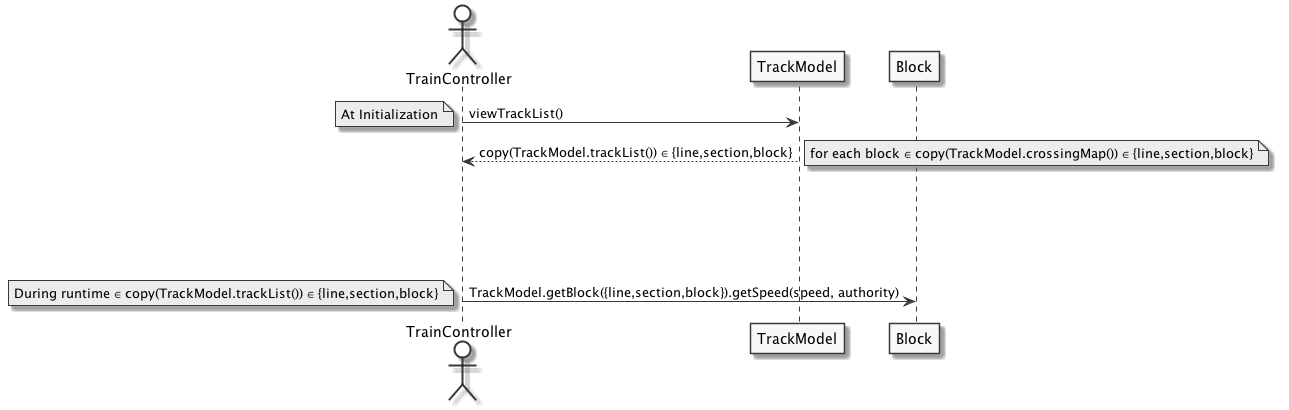
\includegraphics[scale=.3]{getSpeed.png}
	\caption{Get Speed Use Case Diagram}
\end{figure}

\begin{figure}[H]
	\centering
	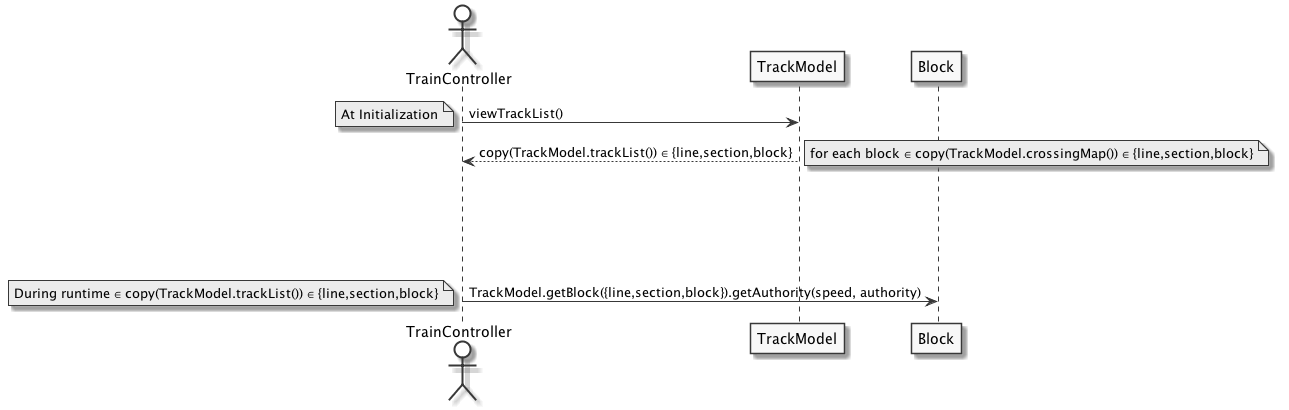
\includegraphics[scale=.3]{getAuthority.png}
	\caption{Get Authority Use Case Diagram}
\end{figure}

\begin{figure}[H]
	\centering
	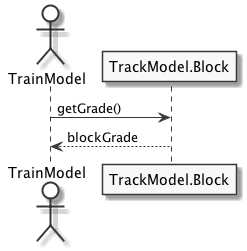
\includegraphics[scale=.3]{getGrade.png}
	\caption{Get Grade Use Case Diagram}
\end{figure}

\begin{figure}[H]
	\centering
	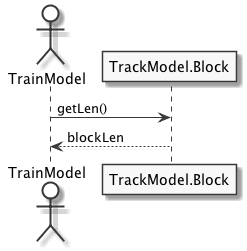
\includegraphics[scale=.3]{getLen.png}
	\caption{Get Length Use Case Diagram}
\end{figure}

\begin{figure}[H]
	\centering
	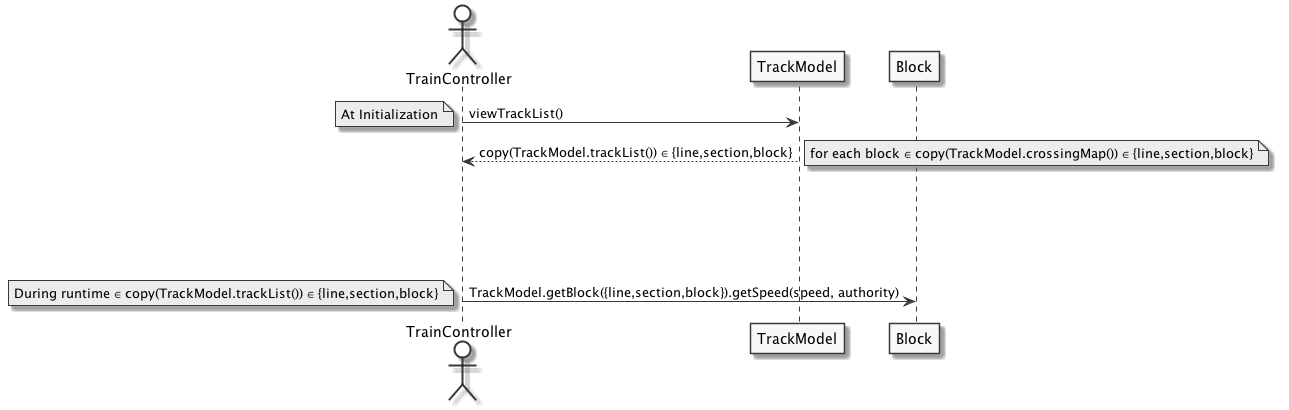
\includegraphics[scale=.3]{getSpeed.png}
	\caption{Get Speed Use Case Diagram}
\end{figure}

\begin{figure}[H]
	\centering
	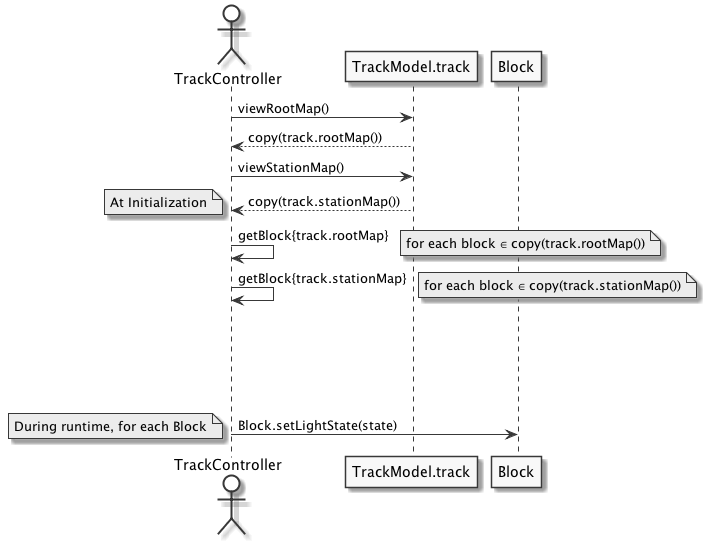
\includegraphics[scale=.3]{lights.png}
	\caption{Toggle Lights Use Case Diagram}
\end{figure}

\begin{figure}[H]
	\centering
	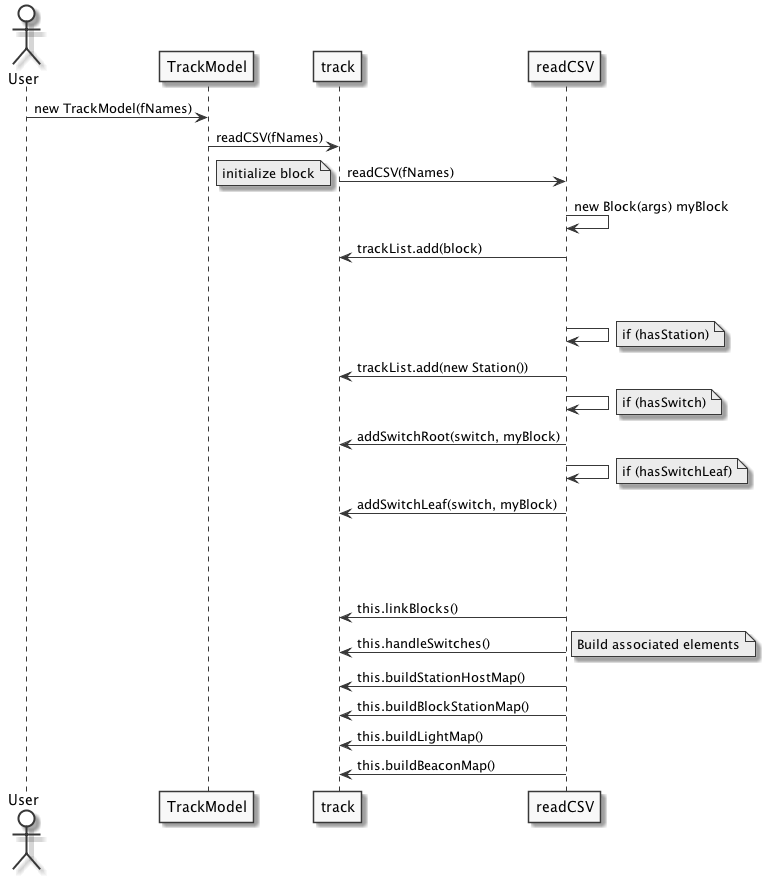
\includegraphics[scale=.3]{readFile.png}
	\caption{Read File Use Case Diagram}
\end{figure}

\subsection{Track Controller}

\subsection{Train Model}
In this seciton, we provide the sequence diagrams of the train model.
\begin{figure}[H]
	\centering
	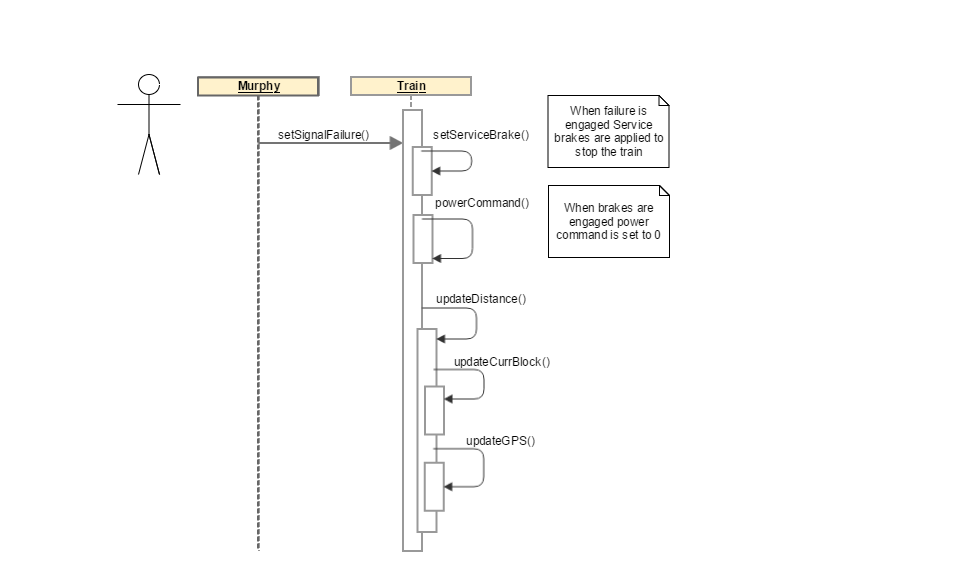
\includegraphics[scale=.3]{train_model_sqd_toggle_signal_failure.png}
	\caption{Toggle Signal Failure Use Case Diagram}
\end{figure}

\begin{figure}[H]
	\centering
	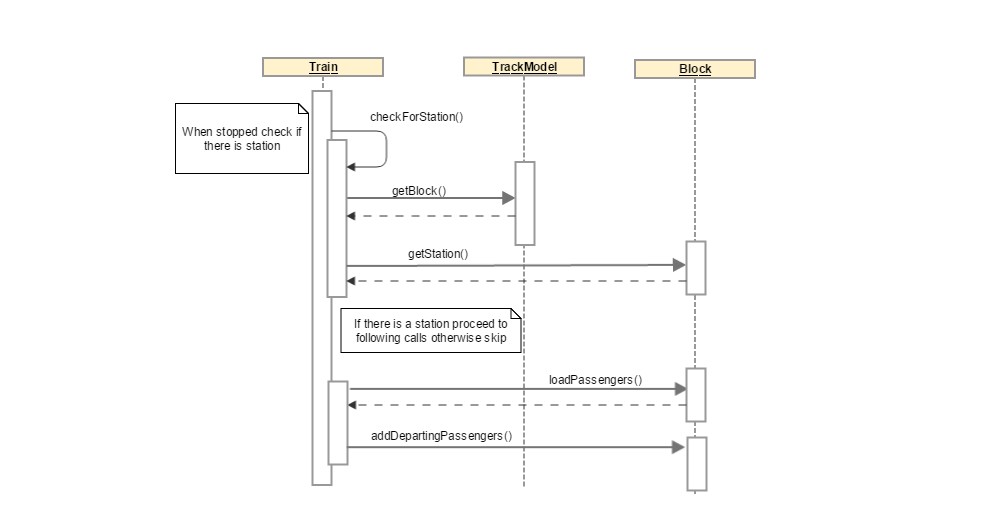
\includegraphics[scale=.3]{train_model_sqd_add_passengers.png}
	\caption{Add Passengers Use Case Diagram}
\end{figure}

\begin{figure}[H]
	\centering
	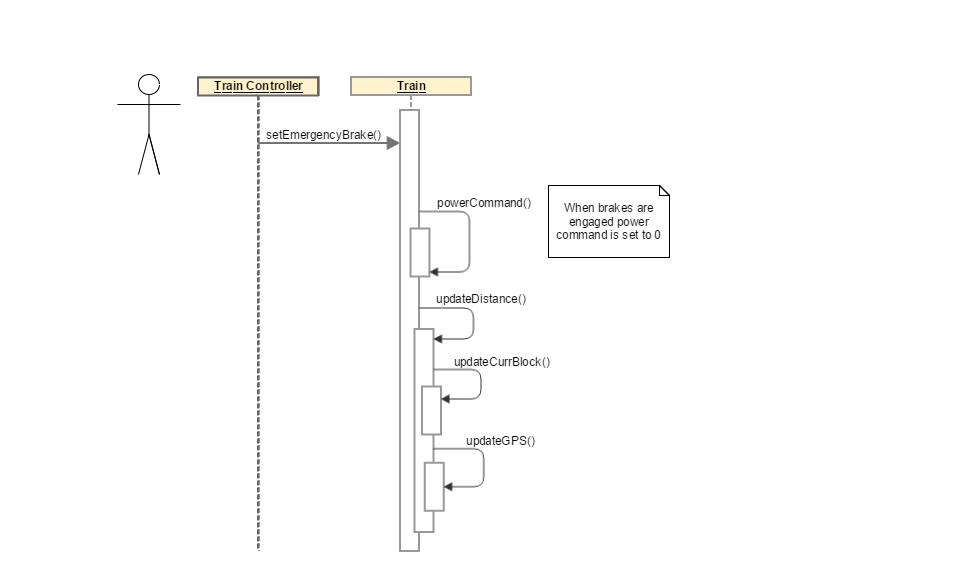
\includegraphics[scale=.3]{train_model_sqd_engage_emergency_brake.png}
	\caption{Engage Emergency Brake Use Case Diagram}
\end{figure}

\begin{figure}[H]
	\centering
	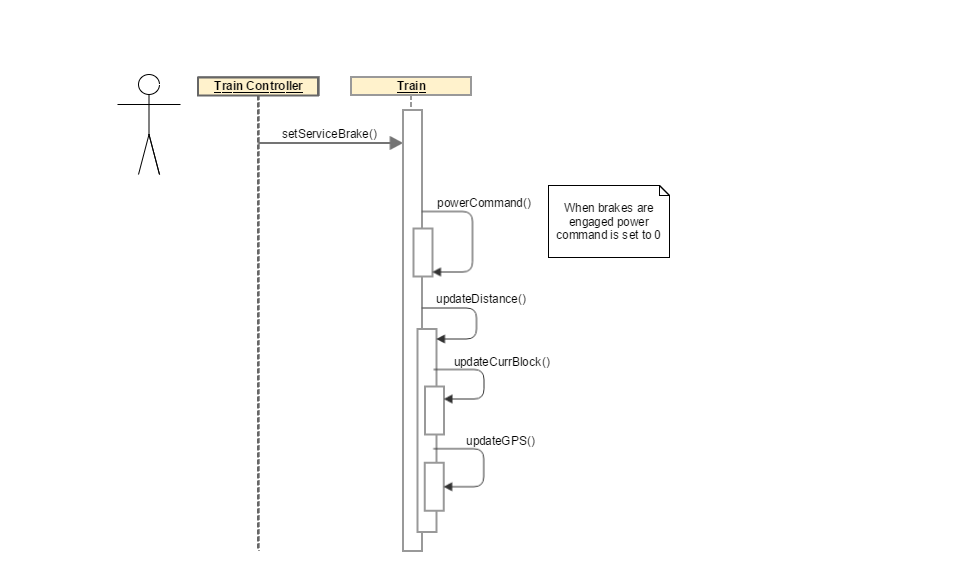
\includegraphics[scale=.3]{train_model_sqd_engage_service_brake.png}
	\caption{Engage Service Brake Use Case Diagram}
\end{figure}

\begin{figure}[H]
	\centering
	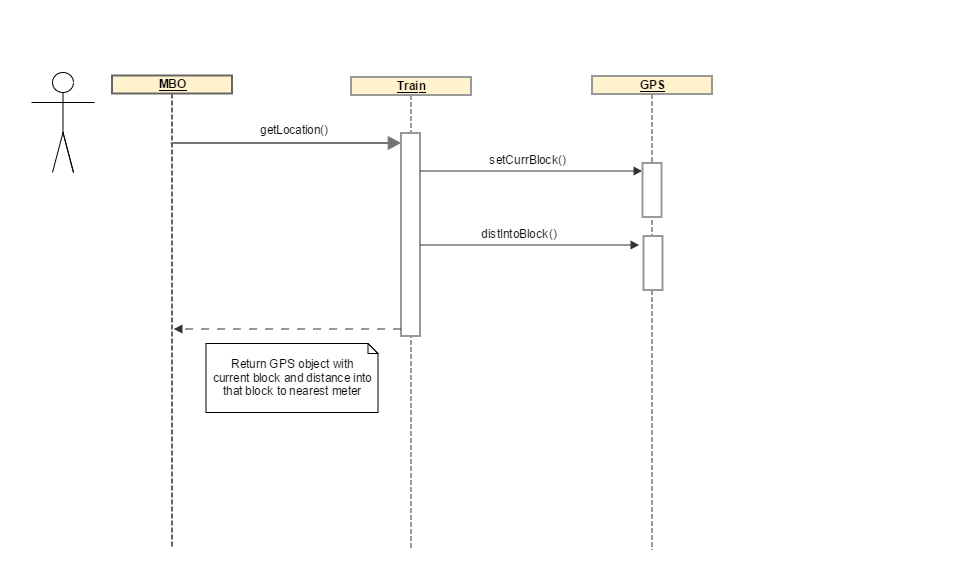
\includegraphics[scale=.3]{train_model_sqd_get_location.png}
	\caption{Get Location Use Case Diagram}
\end{figure}

\begin{figure}[H]
	\centering
	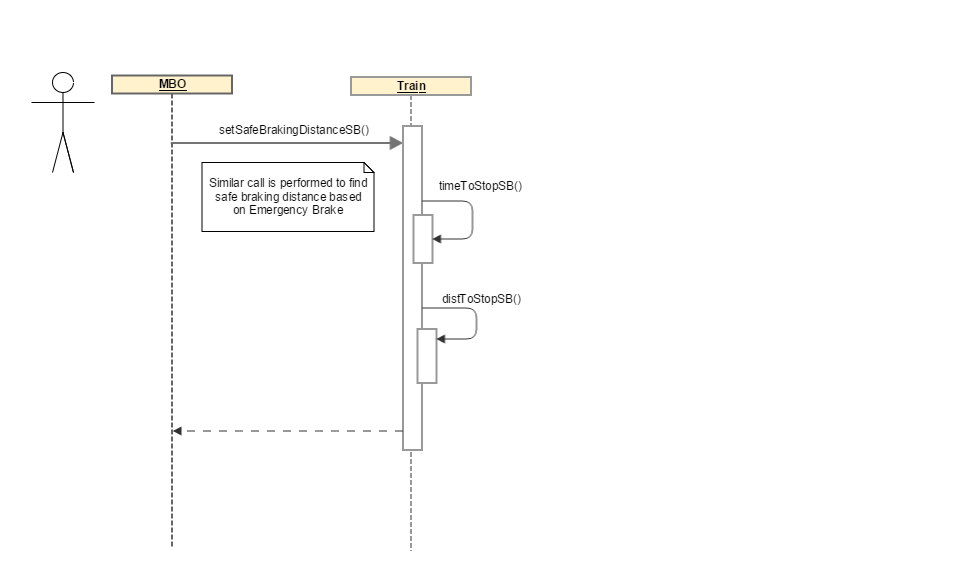
\includegraphics[scale=.3]{train_model_sqd_get_safebraking_dist.png}
	\caption{Calculate Safe Braking Distance Use Case Diagram}
\end{figure}

\begin{figure}[H]
	\centering
	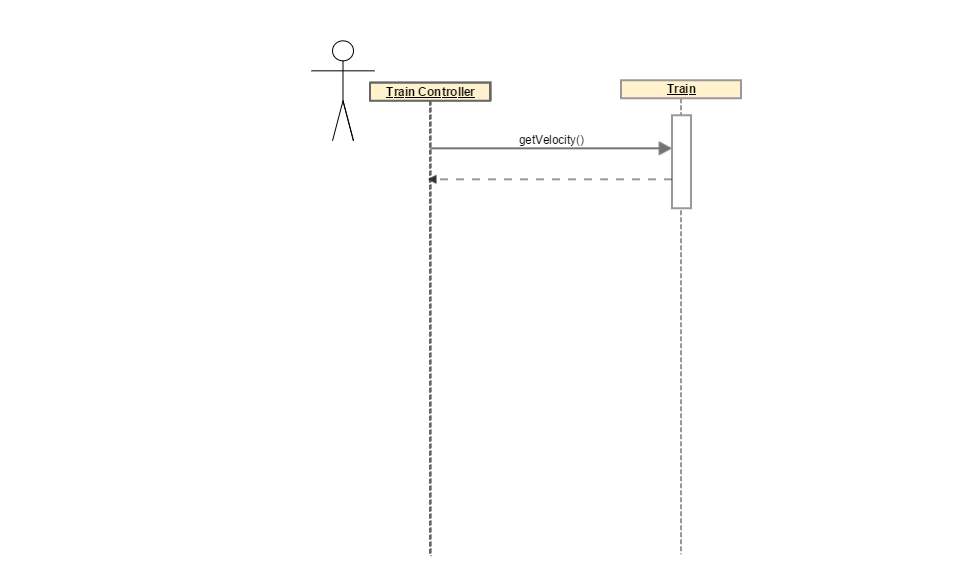
\includegraphics[scale=.3]{train_model_sqd_get_velocity.png}
	\caption{Get Velocity Use Case Diagram}
\end{figure}

\begin{figure}[H]
	\centering
	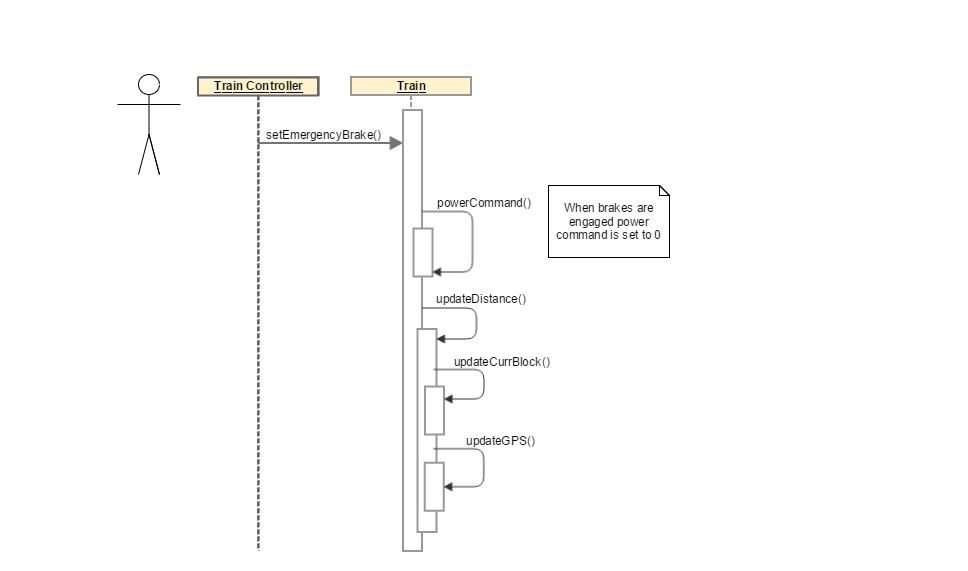
\includegraphics[scale=.3]{train_model_sqd_increase_temp.png}
	\caption{Increase Temperature Use Case Diagram}
\end{figure}

\begin{figure}[H]
	\centering
	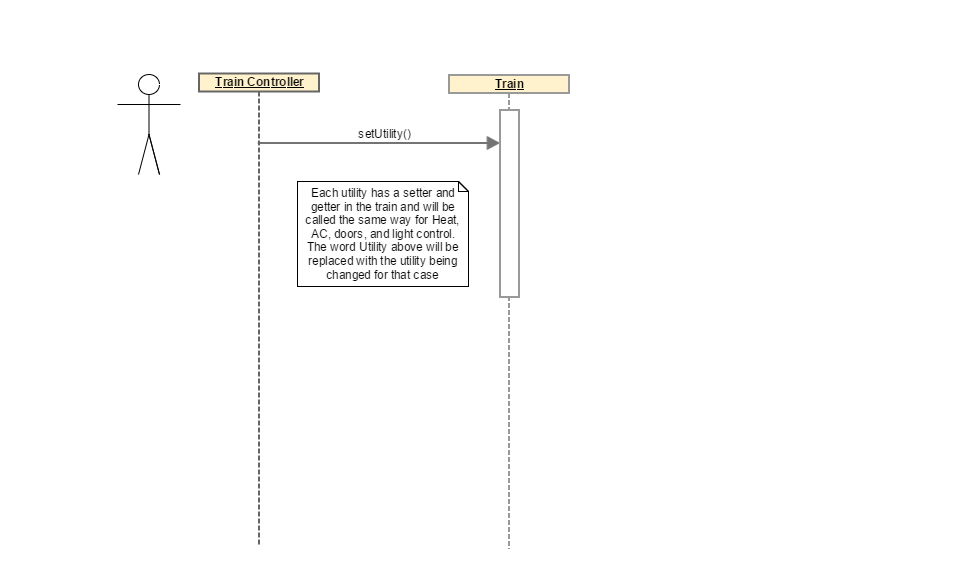
\includegraphics[scale=.3]{train_model_sqd_modify_utlilties.png}
	\caption{Modify Utilities Use Case Diagram}
\end{figure}

\begin{figure}[H]
	\centering
	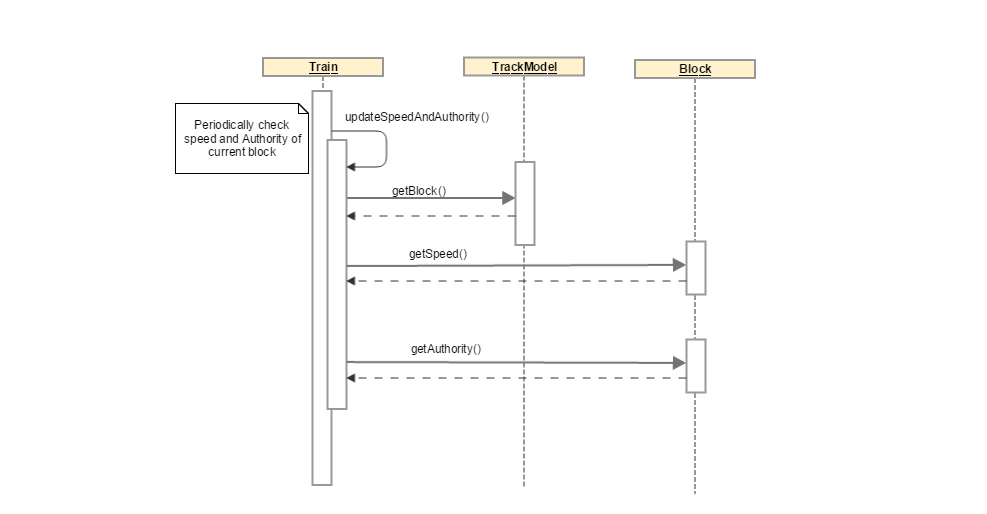
\includegraphics[scale=.3]{train_model_sqd_set_speed_authority.png}
	\caption{Set Speed and Authority Use Case Diagram}
\end{figure}

\begin{figure}[H]
	\centering
	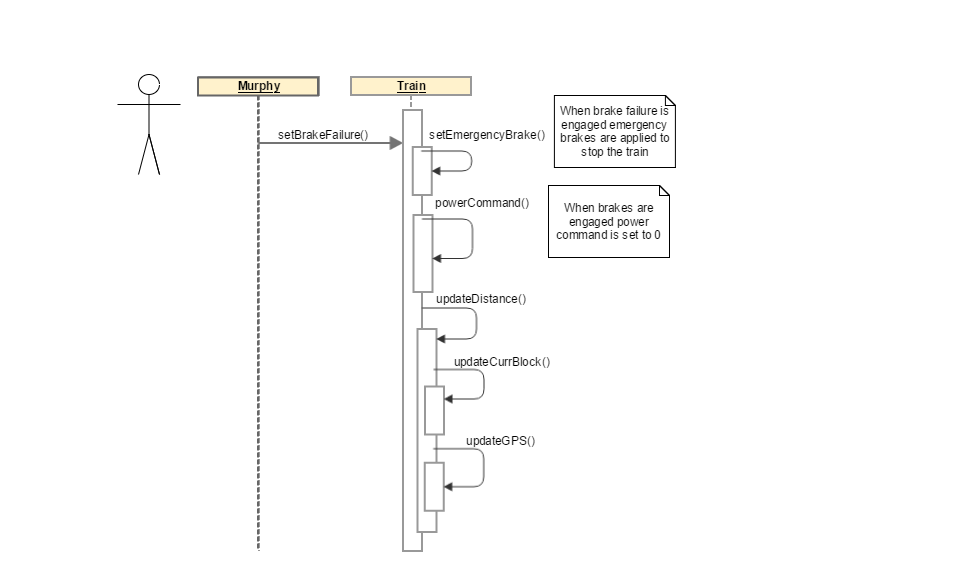
\includegraphics[scale=.3]{train_model_sqd_toggle_brake_failure.png}
	\caption{Toggle Brake Failure Use Case Diagram}
\end{figure}

\begin{figure}[H]
	\centering
	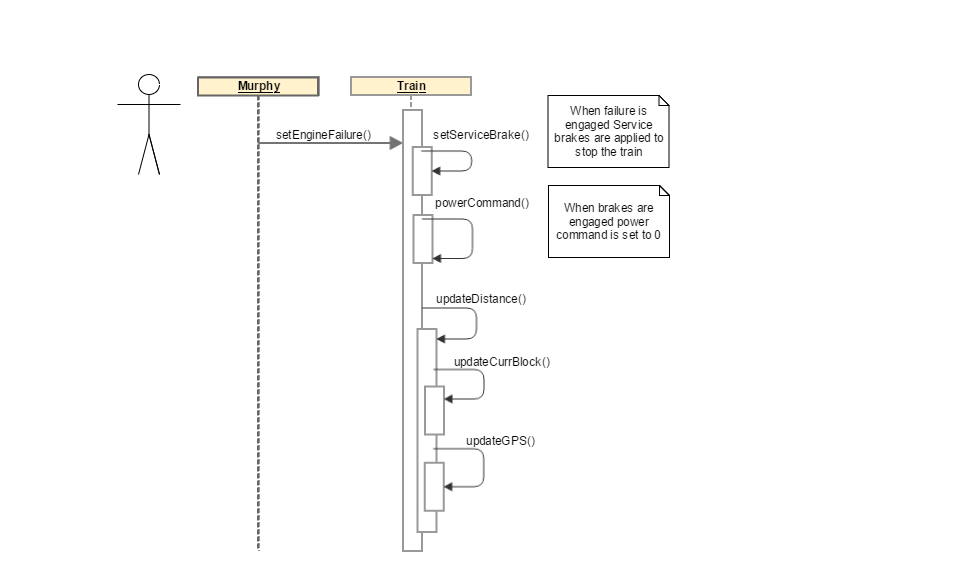
\includegraphics[scale=.3]{train_model_sqd_toggle_engine_failure.png}
	\caption{Toggle Engine Failure Use Case Diagram}
\end{figure}

\begin{figure}[H]
	\centering
	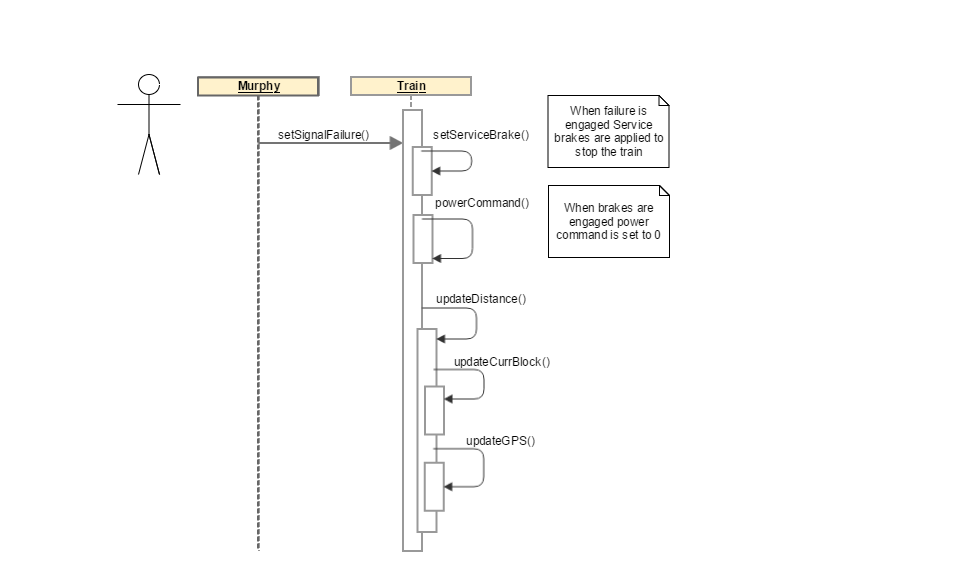
\includegraphics[scale=.3]{train_model_sqd_toggle_signal_failure.png}
	\caption{Toggle Signal Failure Use Case Diagram}
\end{figure}

\begin{figure}[H]
	\centering
	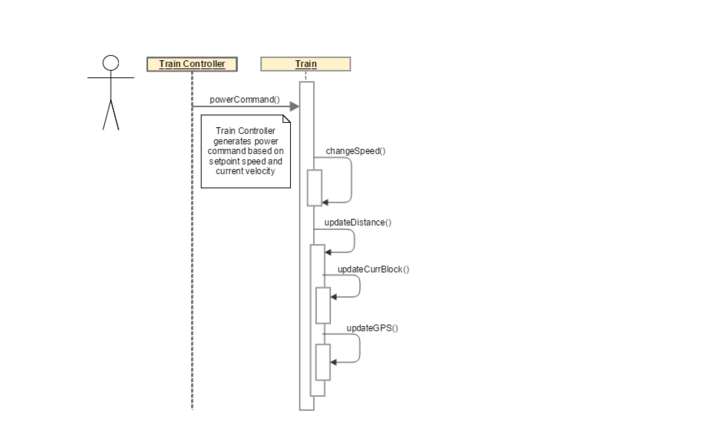
\includegraphics[scale=.3]{train_model_sqd_set_power.png}
	\caption{Toggle Signal Failure Use Case Diagram}
\end{figure}

\subsection{Train Controller}
\subsection{Moving Block Overlay}
\subsection{Centralized Train Controller}


\end{document}          

